\section{Analysis}

\subsection{Task composition}

\subsubsection{Pixel Membership}

From the analysis of the planned Fuzzy Entropy algorithms, one major task to be undertaken would be to calculate the membership of each pixel. Membership stems from Fuzzy set theory, as outlined in Subsection \ref{ssec:fuzzy-entropy}.

There are two common methods to modeling degrees of membership. The first is to manually define the categorty boundaries, so in the case of trapezium functions, the two bases and the two shoulders. The other solution would be to iterate over the values you have and to computationally build the an even distribution throughout your membership functions, as in \cite{Mac_Parthalain_Strange_2013}. Whilst this is the preferred method for being dynamic in it's calculations, it is also more computationally expensive as pre-processing of the image would have to be completed before the Congealing algorithm could be run.

Taking the computational-expense into account, for grey-level pixel values, ranging from 0 (black) to 255 (white), three trapezium functions would be sufficient, therefore modeling `Low', `Medium' and `High' grey-level values. The bases and shoulders would be statically defined, as in Figure \ref{fig:3-traps}. For Non-Probabilistic entropy the highest membership for each pixel from each of the three trapeziums would be taken as the membership degree. Hybrid entropy would take a slightly different approach, which will be covered later.

\begin{figure}[H]
  \center
  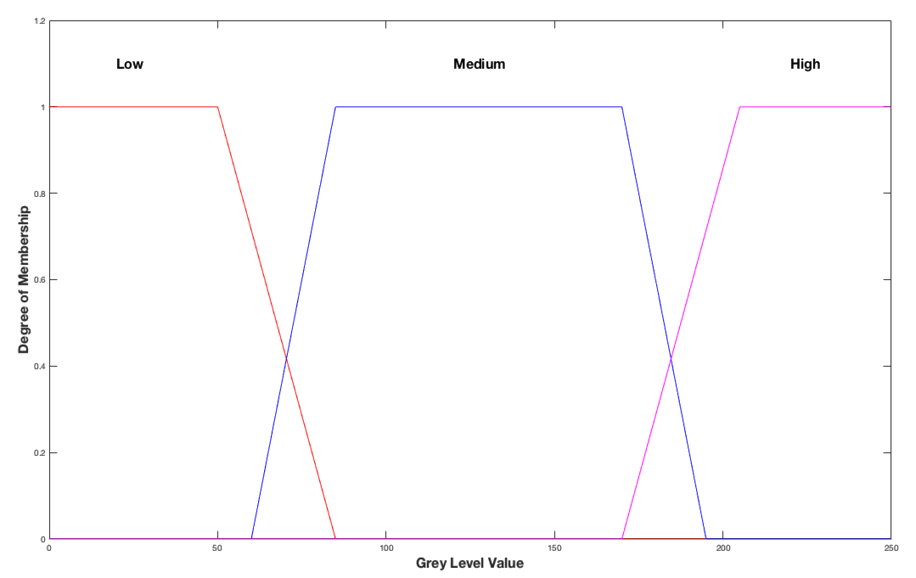
\includegraphics[scale=0.4]{Chapter2/hybrid-img/3_traps.png}
  \caption{3 trapezium-shaped membership sets}
  \label{fig:3-trapeziums}
\end{figure}

\subsubsection{Fuzzy Entropy choices}

\textbf{Chosen algorithms:}
\begin{itemize}
  \item Non-Probability Entropy
  \item Hybrid Entropy
\end{itemize}

Given the simplistic nature of Non-Probabilistic entropy, this was one of the chosen Fuzzy Entropy algorithms to be implemented in the project.

Hybrid entropy was chosen for implementation in this project due to it's hybrid nature (implementing both Probabilistic and Possibilistic uncertainty) and for it's simplification nature - in the absence of fuzziness, then $E_0$ and $E_1$ reduce to $p_0$ and $p_1$ respectively, therefore classical Shannon entropy. This is especially useful in image processing, and other such areas which deal with a lot of noise.

\textbf{Discarded algorithms:}
\begin{itemize}
  \item Fuzzy Shannon Entropy
\end{itemize}

The initial plan was to implement this algorithm in the project - however after further investigation which revealed that Fuzzy Shannon Entropy does not model Probabilistic uncertainty - it was decided that this algorithm was to be excluded.

\subsubsection{Image Alignment choice}

\textbf{Image Alignment choice:}
\begin{itemize}
    \item Congealing
\end{itemize}

As this project will be working with mammograms, something with little variation nor inconsistency, Congealing is the perfect, light-weight image alignment algorithm to which to build upon, especially as the demonstration code available for research has an entropy implementation already developed.

\textbf{Discarded Image Alignment choice:}
\begin{itemize}
    \item Least squares congealing
    \item Joint Alignment of Complex Images
\end{itemize}

Least squares congealing algorithm was disregarded for this project due to the preference to focus upon entropy-based alignment algorithms and the computational costs that the authors themselves regard to be a drawback of their algorithm.

The Complex implementation of Congealing was quickly identified as overly complex for this project. The original Congealing algorithm was more appropriate for grey-scale mammograms, with a consistent canonical pose.

\subsection{Research questions}

The research questions are tightly interwoven with the Objectives of this Project, outlined in Section \ref{sec:objectives}

\begin{itemize}
  \item Does the use of Fuzzy Entropy alignment metrics improve the alignment of mammograms?
  \item Do clinicians / radiographers / mammographers find the output at all useful?
  \item What advantages / disadvantages does each fuzzy entropy alignment metric entail?
\end{itemize}
